%; whizzy paragraph -pdf xpdf -latex ./whizzypdfptex.sh
%; whizzy-paragraph "^\\\\begin{frame}\\|\\\\emtext"
% latex beamer presentation.
% platex, latex-beamer でコンパイルすることを想定。 

%     Tokyo Debian Meeting resources
%     Copyright (C) 2012 Junichi Uekawa

%     This program is free software; you can redistribute it and/or modify
%     it under the terms of the GNU General Public License as published by
%     the Free Software Foundation; either version 2 of the License, or
%     (at your option) any later version.

%     This program is distributed in the hope that it will be useful,
%     but WITHOUT ANY WARRANTY; without even the implied warreanty of
%     MERCHANTABILITY or FITNESS FOR A PARTICULAR PURPOSE.  See the
%     GNU General Public License for more details.

%     You should have received a copy of the GNU General Public License
%     along with this program; if not, write to the Free Software
%     Foundation, Inc., 51 Franklin St, Fifth Floor, Boston, MA  02110-1301 USA

\documentclass[cjk,dvipdfmx,12pt]{beamer}
\usetheme{Tokyo}
\usepackage{monthlypresentation}

%  preview (shell-command (concat "evince " (replace-regexp-in-string "tex$" "pdf"(buffer-file-name)) "&")) 
%  presentation (shell-command (concat "xpdf -fullscreen " (replace-regexp-in-string "tex$" "pdf"(buffer-file-name)) "&"))
%  presentation (shell-command (concat "evince " (replace-regexp-in-string "tex$" "pdf"(buffer-file-name)) "&"))

%http://www.naney.org/diki/dk/hyperref.html
%日本語EUC系環境の時
\AtBeginDvi{\special{pdf:tounicode EUC-UCS2}}
%シフトJIS系環境の時
%\AtBeginDvi{\special{pdf:tounicode 90ms-RKSJ-UCS2}}

\newenvironment{commandlinesmall}%
{\VerbatimEnvironment
  \begin{Sbox}\begin{minipage}{1.0\hsize}\begin{fontsize}{8}{8} \begin{BVerbatim}}%
{\end{BVerbatim}\end{fontsize}\end{minipage}\end{Sbox}
  \setlength{\fboxsep}{8pt}
% start on a new paragraph

\vspace{6pt}% skip before
\fcolorbox{dancerdarkblue}{dancerlightblue}{\TheSbox}

\vspace{6pt}% skip after
}
%end of commandlinesmall

\title{Debian JP Project / \\東京エリアDebian勉強会}
\subtitle{OSC2016 群馬 出張版}
\author{岩松 信洋}
\date{2016年5月14日}
\logo{
\includegraphics[width=8cm]{image200607/openlogo-light.eps}}

\begin{document}

\begin{frame}
\titlepage{}
\end{frame}


\begin{frame}{自己紹介}

\begin{itemize}
\item 名前: 岩松 信洋(いわまつ のぶひろ)
\item Debian Project Official Developer
\item Debian でのお仕事: Debian linux kernel, Debian Bluetooth, Debian Science (OpenCV), Erlang, Debian Go
\item 普段のお仕事: Linux kernel 開発、U-Boot メンテナ、Yocto Project
\end{itemize} 
\end{frame}

\begin{frame}{Agenda}
  \begin{itemize}
   \item Debian とは?
   \item Debian Updates
   \item 今後のイベント
  \end{itemize}
\end{frame}

\section{Debian とは?}
\begin{frame}\begin{center}\Huge{Debian とは?}\end{center}\end{frame}

\begin{frame}{Debian とは?}
フリー/オープンなオペレーティングシステム (OS)を作成しようとするボランティアベースのプロジェクト。

\begin{table}[htb]
  \begin{tabular}{|c|c|c|}
    \hline
    ディストリ & 企業 & ボランティア \\ \hline
    RHEL & RedHat & なし  \\ \hline
    CentOS & RedHat & あり \\ \hline
    Ubuntu  & Canonical & あり \\ \hline
    \color{red}{Debian}  & \color{red}{なし} & \color{red}{あり} \\ \hline
  \end{tabular}
\end{table}

\end{frame}

\begin{frame}{Debian とは?}
Linux カーネルだけではなく、FreeBSD や GNU/Hurd のカーネルを利用したOSも提供。

 \begin{center}
% \includegraphics[width=0.3\hsize]{image201605/Freebsd-logo.png}
% \includegraphics[width=0.4\hsize]{image201605/hurd.png}
 \end{center}

\end{frame}

\begin{frame}{Debian とは?}
\begin{itemize}[<+->]
\item Debian 社会契約(オープンソースの定義の元)、Debian フリーソフトウェアガイドライン、Debian Policy
\item Ubuntu や Raspbian といったディストリビューションのベースとなっている
 \begin{center} 
 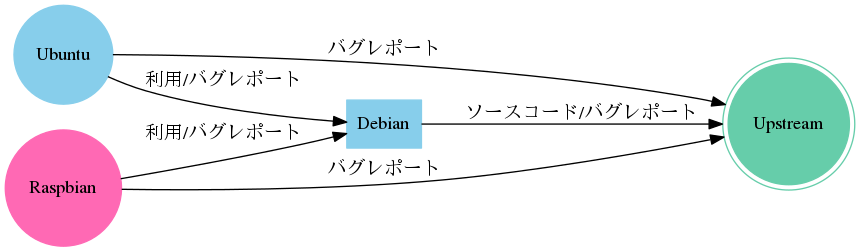
\includegraphics[width=0.8\hsize]{image201605/debian_derivatives.png}
 \end{center} 
\end{itemize}
\end{frame}

\begin{frame}{Debian とは?}
 世界規模で開発が行われており、63ヶ国、約1000名のDebian公式開発者が開発を行
 っている。パッケージメンテナや翻訳などの貢献者も入れるともっと多くの開発者が参加
 していることになる。
% \begin{center}
% \includegraphics[width=0.7\hsize]{image201605/debconf15_group.jpg}
% \end{center}
\end{frame}

\begin{frame}{Debian とは?}
\begin{itemize}[<+->]
 \item 2016年5月の時点で、\pause 最新版は Debian 8.4 (コードネーム Jessie)、\pause パッケージ数は約43000を提供、\pause
 公式にサポートするCPUアーキテクチャは10。\pause
 \item 約2年毎にリリース
% \begin{center}
% \includegraphics[width=0.7\hsize]{image201605/a55b040cecdfc1bc7f9d81a1fc7e0f6a.png}
% \end{center}
 \item 次のリリース (コードネーム: Stretch)は 2018年Q2またはQ3の予定
 \item コードネームはトイ・ストーリのキャラクターを採用している。
\end{itemize}
\end{frame}


\begin{frame}{Debian とは?}
どこで使われているのか?\pause
Webサーバとして利用されてる(2016/01時点)

%  \begin{center}
%  \includegraphics[width=0.5\hsize]{image201605/w3techs.png}
%  \end{center}
  \tiny{\url{http://w3techs.com/technologies/details/os-linux/all/all}}

\end{frame}

\begin{frame}{Debian とは?}
組込デバイスのベースOSとして利用されている

% \begin{center}
% \includegraphics[width=0.2\hsize]{image201605/hp_black_sm.jpg}
% \end{center}
 \url{http://beagleboard.org/}

% \begin{center}
% \includegraphics[width=0.2\hsize]{image201605/raspberry-pi-logo.png}
% \end{center}
 \url{https://www.raspberrypi.org/}

 \end{frame}

\begin{frame}{Debian とは?}

\begin{itemize}
\item ISS (国際宇宙ステーション)
%\begin{center}
%\includegraphics[width=0.5\hsize]{image201605/ISS.jpg}
%\end{center}

\item Steam (ゲームPC OS)
\item NAS、ルータ
\item etc..
\end{itemize}

\end{frame}
\begin{frame}{Debian とは?}
まとめると\pause
\begin{itemize}[<+->]
\item Debianはフリー/オープンなオペレーティングシステム (OS)を作成しようとするボランティアベースのプロジェクト。
\item 自分たちの考えるフリーという言葉に関する定義、開発目的、パッケージングポリシーを厳格に決めている。
\item 世界中に1000人以上の開発者がおり、他のディストリビューションのベースとして採用されている。
\item 約2年毎にリリースが行われ、多くのパッケージとアーキテクチャをサポートしている。次期リリースは2018年Q2からQ3。
\item 上記のような特徴から様々なところで利用されているLinuxディストリビューションである。
\end{itemize}

\end{frame}

\begin{frame}{Debian JP Project とは?}
\pause
\begin{itemize}[<+->]
\item 日本でDebianを普及させることを目的とした任意団体。
\item Debian の日本語による情報発信、ユーザとの情報交換、Debian 開発者の育成など
\item 東京エリアDebian勉強会は東京近辺在住のDebian開発者、ユーザによる勉強会。
\item 東京の他、関西でも同様の勉強会が行われている。
\item 月に一回開催中。
\end{itemize}

\end{frame}

\section{Debian Updates}
\begin{frame}\begin{center}\Huge{Debian Updates}\end{center}\end{frame}

\begin{frame}{Debian Updates}% [containsverbatim]

\begin{itemize}[<+->]
\item 2016/02/29: Debian 6 Long Term Support (LTS)終了\\
   \pause \small{LTSチームが利用企業からスポンサー支援を受け、i386, amd64, armelとarmhf
   のアーキテクチャに対してセキュリティアップデートを行う。\\
   期間は対象リリースのセキュリティサポートが切れてから約2年間。Debian 7 は 2016年4月26日にサポートが切れたので、
   2018年5月31日まで。}
   \pause
\item 2016/04/02: Updated Debian 8: 8.4, Debian 7: 7.10
\item 2016/04/25: Debian 7.0(Wheezy) のセキュリティサポートが LTS チームに移行
\item 2016/05/07: 次期リリース版である Debian 9 の i386アーキテクチャのサポートCPUをi686以降に変更
\end{itemize}

\end{frame}

\section{日本語によるDebianの情報}
\begin{frame}\begin{center}\Huge{日本語によるDebianの情報}\end{center}\end{frame}

\begin{frame}{日本語によるDebianの情報}
\begin{itemize}
  \item Debian JP Project \\
      \url{http://www.debian.or.jp}
  \item 東京エリアDebian勉強会\\
      \url{http://tokyodebian.alioth.debian.org}
  \item 関西エリアDebian勉強会 \\
      \url{https://wiki.debian.org/KansaiDebianMeeting}
  \item Twitter \\
      \url{@debian_jp}
  \item G+ コミュニティ \\
      \url{https://plus.google.com/u/0/communities/106942835439686570073}
 
\end{itemize}
\end{frame}

\section{今後のイベント}
\begin{frame}\begin{center}\Huge{今後のイベント}\end{center}\end{frame}

\begin{frame}{今後のイベント}
\begin{itemize}
\item 5月21日 第110回関西Debian勉強会
  \begin{itemize}
      \item 福島区民センター304号会議室
      \item \url{https://wiki.debian.org/KansaiDebianMeeting/20160521}
  \end{itemize}
\item 5月21日 第139回東京エリアDebian勉強会
  \begin{itemize}
      \item 朝日ネットさん(東京/銀座)
      \item \url{http://tokyodebian.alioth.debian.org/2016-05.html}
  \end{itemize}

\item 6月17-18日 OSC2016 北海道 セミナーおよび出展

\end{itemize}
\end{frame}

\begin{frame}{質問}
\begin{center}
何か質問はありますか?
\end{center}
\end{frame}

%\begin{frame}{利用画像}
%  \begin{itemize}
%  \item image201605/w3techs.png:
%    \url{https://plus.google.com/+CybercitiBiz/posts/FS4FPZmGAeK}
%  \end{itemize}
%\end{frame}
%
\end{document}

;;; Local Variables: ***
;;; outline-regexp: "\\([ 	]*\\\\\\(documentstyle\\|documentclass\\|emtext\\|section\\|begin{frame}\\)\\*?[ 	]*[[{]\\|[]+\\)" ***
;;; End: ***
